

% Prepared by Calvin Kent
%
% Assignment Template v19.02
%
%%% 20xx0x/MATHxxx/Crowdmark/Ax
%
\documentclass[12pt]{article} %
\usepackage{CKpreamble}
\usepackage{CKassignment}
\usepackage{tkz-euclide}
\usepackage{physunits}
\usepackage{physics}
\usepackage{lmodern}
\usepackage{microtype}
\usepackage{upgreek}
\usepackage[misc]{ifsym}


%%Title
\title{Functions Quiz 1}
\date{November, 2021}

%%% Maths and science packages

\usepackage{amsmath,amsthm,amssymb}
\usepackage{pgfplots}
	\usetikzlibrary{
		calc,
		patterns,
		positioning
	}
	\pgfplotsset{
		compat=1.16,
		samples=200,
		clip=false,
		my axis style/.style={
			axis x line=middle,
			axis y line=middle,
			legend pos=outer north east,
			axis line style={
				->,
			},
			legend style={
				font=\footnotesize
			},
			label style={
				font=\footnotesize
			},
			tick label style={
				font=\footnotesize
			},
			xlabel style={
				at={
					(ticklabel* cs:1)
				},
				anchor=west,
				font=\footnotesize,
			},
			ylabel style={
				at={
					(ticklabel* cs:1)
				},
				anchor=west,
				font=\footnotesize,
			},
			xlabel= $x$,
			ylabel=$\vec d (\m \tx{[East]})$
		},
	}
	\tikzset{
		>=stealth
	}

%%% Tables and figures packages

\usepackage{float}
\usepackage{caption}
	\captionsetup{
		format=plain,
		labelfont=bf,
		font=small,
		justification=centering
	}
	
%%% Numbers and sets

\newcommand{\E}{\mathrm{e}}

\newcommand{\tx}[1]{\text{#1}}

\begin{document}
    \pagenumbering{arabic}
    % Start of class settings ...
    \renewcommand*{\coursecode}{MCR3U Quiz} % Quiz Title
    \renewcommand*{\assgnnumber}{1} % Quiz number
    \renewcommand*{\submdate}{November, 2021} % renew the date
    \renewcommand*{\studentfname}{\textbf{Name:}} % Student first name
    \renewcommand*{\studentlname}{} % Student last name
    %\renewcommand*{\studentnum}{SNumber} % Student number

    \renewcommand\qedsymbol{$\blacksquare$}
    \setfigpath
    % End of class settings 
    \pagestyle{crowdmark}
    \newgeometry{left=18mm, right=18mm, top=22mm, bottom=22mm} % page is set to default values
    \fancyhfoffset[L,O]{0pt} % header orientation fixed
    % End of class settings
    %%% Note to user:
    % CTRL + F <CHANGE ME:> (without the angular brackets) in CKpreamble to specify graphics paths accordingly.
    % The command \circled[]{} accepts one optional and one mandatory argument.
    % Optional argument is for the size of the circle and mandatory argument is for its contents.
    % \circled{A} produces circled A, with size drawn for letter A. \circled[TT]{A} produces circled A with size drawn for TT.
    % https://github.com/CalvinKent/My-LaTeX
    %%%
    % Crowdmark assignment start


    %%%%%%%%%%%%%%%%%%%%%%%%%%%%%%%%%%%%%%%%%%%%%%%%%%%%%%%%%%%%%%%%%%%%%%%%%%%%%%%%%%%%%%%%%%%%%%%%%%%%%%%%
    %%%%%%%%%%%%%%%%%                  PROBLEM IDEAS                  %%%%%%%%%%%%%%%%%%%%%%%%%%%%%%%%%%%%%%
    %%%%%                   ----------------------------------------                                %%%%%%%%

    % --> Do a hard tangent line problem

\begin{qstn}[1] % qnumber, qname, qpoints
  Answer the following True/False questions,
  \begin{enumerate}
    \item The two fundamental properties of sets are,
      \begin{itemize}
        \item Duplicate elements are not allowed.
        \item Order matters.
      \end{itemize}
      \textbf{\emph{Answer}}: \,\,\, \textbf{False}, \,\, The order \emph{does not} matter.\\



    \item Let $S = \{3,4,5,2,1,3,0\} $, then $(-3+4-5+2-1+3) \in S$.\\
      \textbf{\emph{Answer}}: \,\,\, \textbf{True},\,\, Observe that $-3+4-5+2-1+3 = 0$ and $0 \in S$, so its true.\\


    \item $\sqrt{4} \in \Z$.\\
      \textbf{\emph{Answer}}: \,\,\, \textbf{True},\,\, $\sqrt{4} = 2$ and $2\in \Z$.\\



    \item The vertex of 
      \[
        f(x) = 3\left( x + 4 \right)^2 + 1 
      \] is (4,1).\\ 
      \textbf{\emph{Answer}}: \,\,\, \textbf{False},\,\, The vertex here is $(-4,1)$.\\



    \item The centre of the circle,
      \[
            (x+1)^2 + (y +2)^2 = 4
      \] is $(-1,-2)$.\\
      \textbf{\emph{Answer}}: \,\,\, \textbf{True}\\


    \item The vertex of,
      \[
            f(x) = -\frac{5}{3}\left( x - 3 \right)^2 - 4
      .\] represents a minimum.\\
      \textbf{\emph{Answer}}: \,\,\, \textbf{False},\,\, Since $a = -\frac{5}{3} < 0$, the vertex must represent a maximum.\\

    \item The y-intercept of,
      \[
              f(x) = -x^2 + 3x + 4
      .\] is $-4$.\\
      \textbf{\emph{Answer}}: \,\,\, \textbf{False},\,\, The y-intercept here is $4$.
  \end{enumerate}
\end{qstn}



\begin{qstn}[2]
  Write down the elements of the following sets. (Remember to use dots (\dots) where applicable)
  \begin{enumerate}[label=(\alph*)]
    \item $A = \{t\in \Z \mid 0 \leq  t < 5\} $ 
      \begin{solution}
        $A = \{0,1,2,3,4\} $
      \end{solution}
      
      \vspace*{4cm}

    \item $R = \{r \in \Z \mid r \geq 1\} $ 
      \begin{solution}
        $R = \{1,2,3,4,5,\dots\} $
      \end{solution}
      
      \vspace*{4cm}

    \item $T = \{x \in \Z \mid x^2 = 1\} $
      \begin{solution}
        $T = \{-1,1\} $
      \end{solution}
  \end{enumerate}
\end{qstn}


\begin{qstn}[3]
  Graph the following circle,
  \[
          (x-6)^2 + (y + 8)^2 = 36
  .\] 
    \begin{center}
        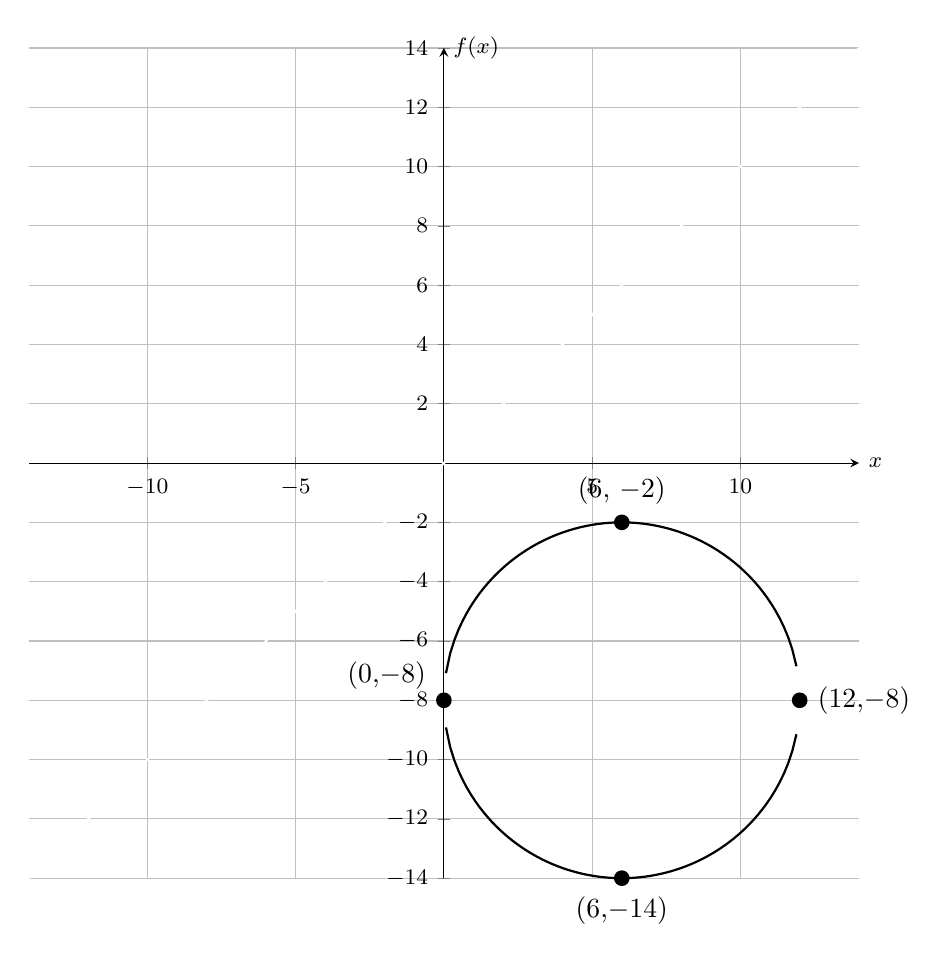
\begin{tikzpicture}
        \begin{axis}[
            my axis style,
            width=\textwidth,
            height=\textwidth,
            ylabel=$f(x)$,
            grid
        ]
        
        \addplot[
            domain=-14:14,
            thick,
            black,
            -
        ]
        {sqrt(-(x-6)^2+36) - 8};

        \addplot[
            domain=-14:14,
            thick,
            white,
            -
        ]
        {x};

        \addplot[
            domain=-14:14,
            thick,
            black,
            -
        ]
        {-1 * sqrt(-(x-6)^2+36) - 8};

        \fill[
            black
        ];

        \node[label={90:{($6$, $-2$)}},circle,fill,inner sep=2pt] at (axis cs:6,-2) {};
        \node[label={170:{($0$,$-8$)}},circle,fill,inner sep=2pt] at (axis cs:0,-8) {};
        \node[label={270:{($6$,$-14$)}},circle,fill,inner sep=2pt] at (axis cs:6,-14) {};
        \node[label={360:{($12$,$-8$)}},circle,fill,inner sep=2pt] at (axis cs:12,-8) {};
 

        \end{axis}
        \end{tikzpicture}
    \end{center}
\end{qstn}


\begin{qstn}[4]
  Lets define the following function,
  \begin{align*}
    f &\colon \R \to \R\\
    f(x) &= -x^2 + 2x + 8
  \end{align*}

 \begin{enumerate}[label=(\alph*)]
      \item Complete the square to convert $f$ into vertex form.
        \begin{solution}
          \begin{step}
            \begin{align*}
               0 &= b^2 - 4at\\
               0 &= 4 - 4(-1)(t)\\
               0 &= 4 + 4t\\
               4t &= -4\\
               t &= -1
            \end{align*}
          \end{step}

          \vspace*{-1cm}

          \begin{step}
            \begin{align*}
              f(x) &= -x^2 + 2x + t -t + 8\\
                   &= -x^2 + 2x + (-1) - (-1) + 8\\
                   &= \left( -x^2 + 2x + (-1) \right) + \left[ 8 - (-1) \right]\\
                   &= -\left( x^2 +\frac{2}{-1}x + \frac{(-1)}{-1} \right) + \left[ 8 + 1 \right] \\
            \end{align*}
          \end{step}

          \vspace*{-1cm}

          \begin{step}
            Since $a \cdot b = -1 \cdot 2 = -2$ we conclude that $a \cdot b < 0$, so we proceed with the following replacement,
            \begin{align*}
              f(x) &= -\left( x - \sqrt{\frac{t}{a}}\right)^2 + 9\\
                   &= -\left( x - \sqrt{\frac{-1}{-1}}  \right)^2 + 9\\
                   &= -\left( x - \sqrt{\frac{1}{1}}  \right)^2 + 9\\
                   &= -\left( x - 1 \right)^2  +9
            \end{align*}
          \end{step}

          \begin{step}
            Finally, we have $f$ in vertex form,
            \[
                  f(x) = -(x-1)^2 + 9
            .\] 
          \end{step}
        \end{solution}
        \newpage
      \item Sketch the function using your answer from part (a) \\(\textbf{NOTE:} Make sure you label the y-intercept as well as the vertex).
 \end{enumerate}
    \begin{center}
        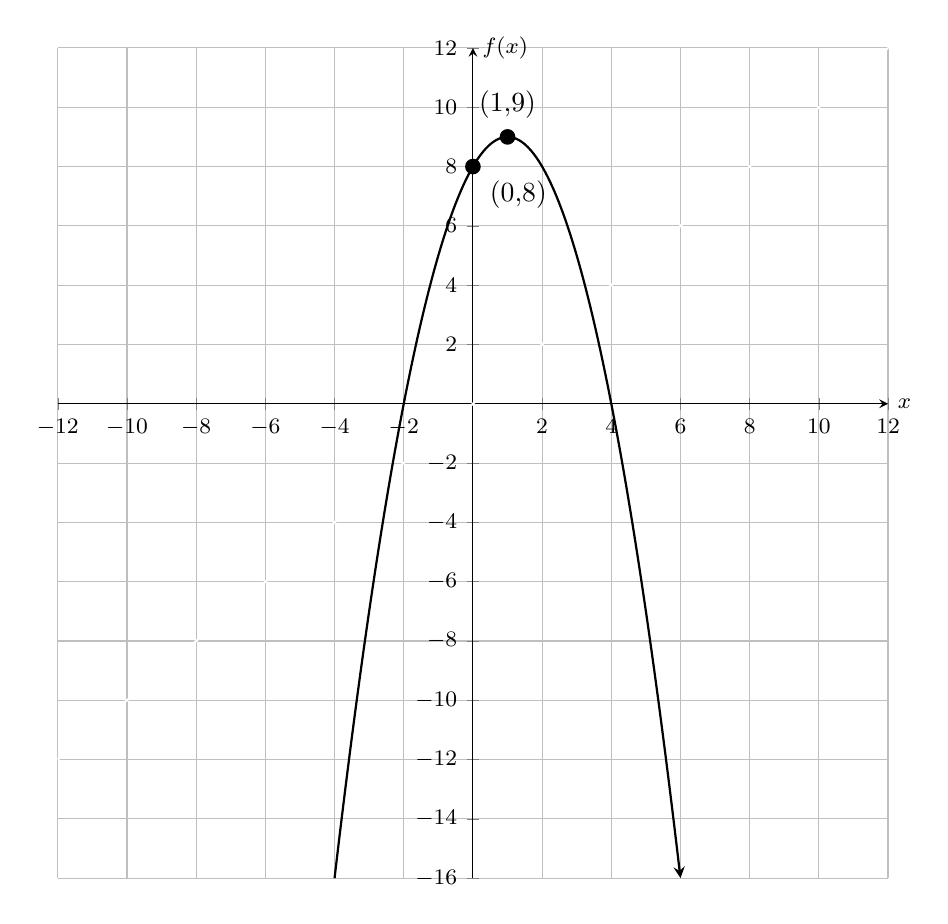
\begin{tikzpicture}
        \begin{axis}[
            my axis style,
            width=\textwidth,
            height=\textwidth,
            ylabel=$f(x)$,
            grid
        ]
        
        \addplot[
            domain=-12:12,
            thick,
            white,
            -
        ]
        {x};

        \addplot[
            domain=-4:6,
            thick,
            black,
            ->
        ]
        {-(x-1)^2 + 9};

        \fill[
            black
        ];


        \node[label={90:{($1$,$9$)}},circle,fill,inner sep=2pt] at (axis cs:1,9) {};
        \node[label={330:{($0$,$8$)}},circle,fill,inner sep=2pt] at (axis cs:0,8) {};
     

        \end{axis}
        \end{tikzpicture}
    \end{center}
\end{qstn}





























\end{document}
